\subsection{Experiment 5: Characteristics of Metrics in Classification Tasks}

\begin{figure}[H]
    \centering
    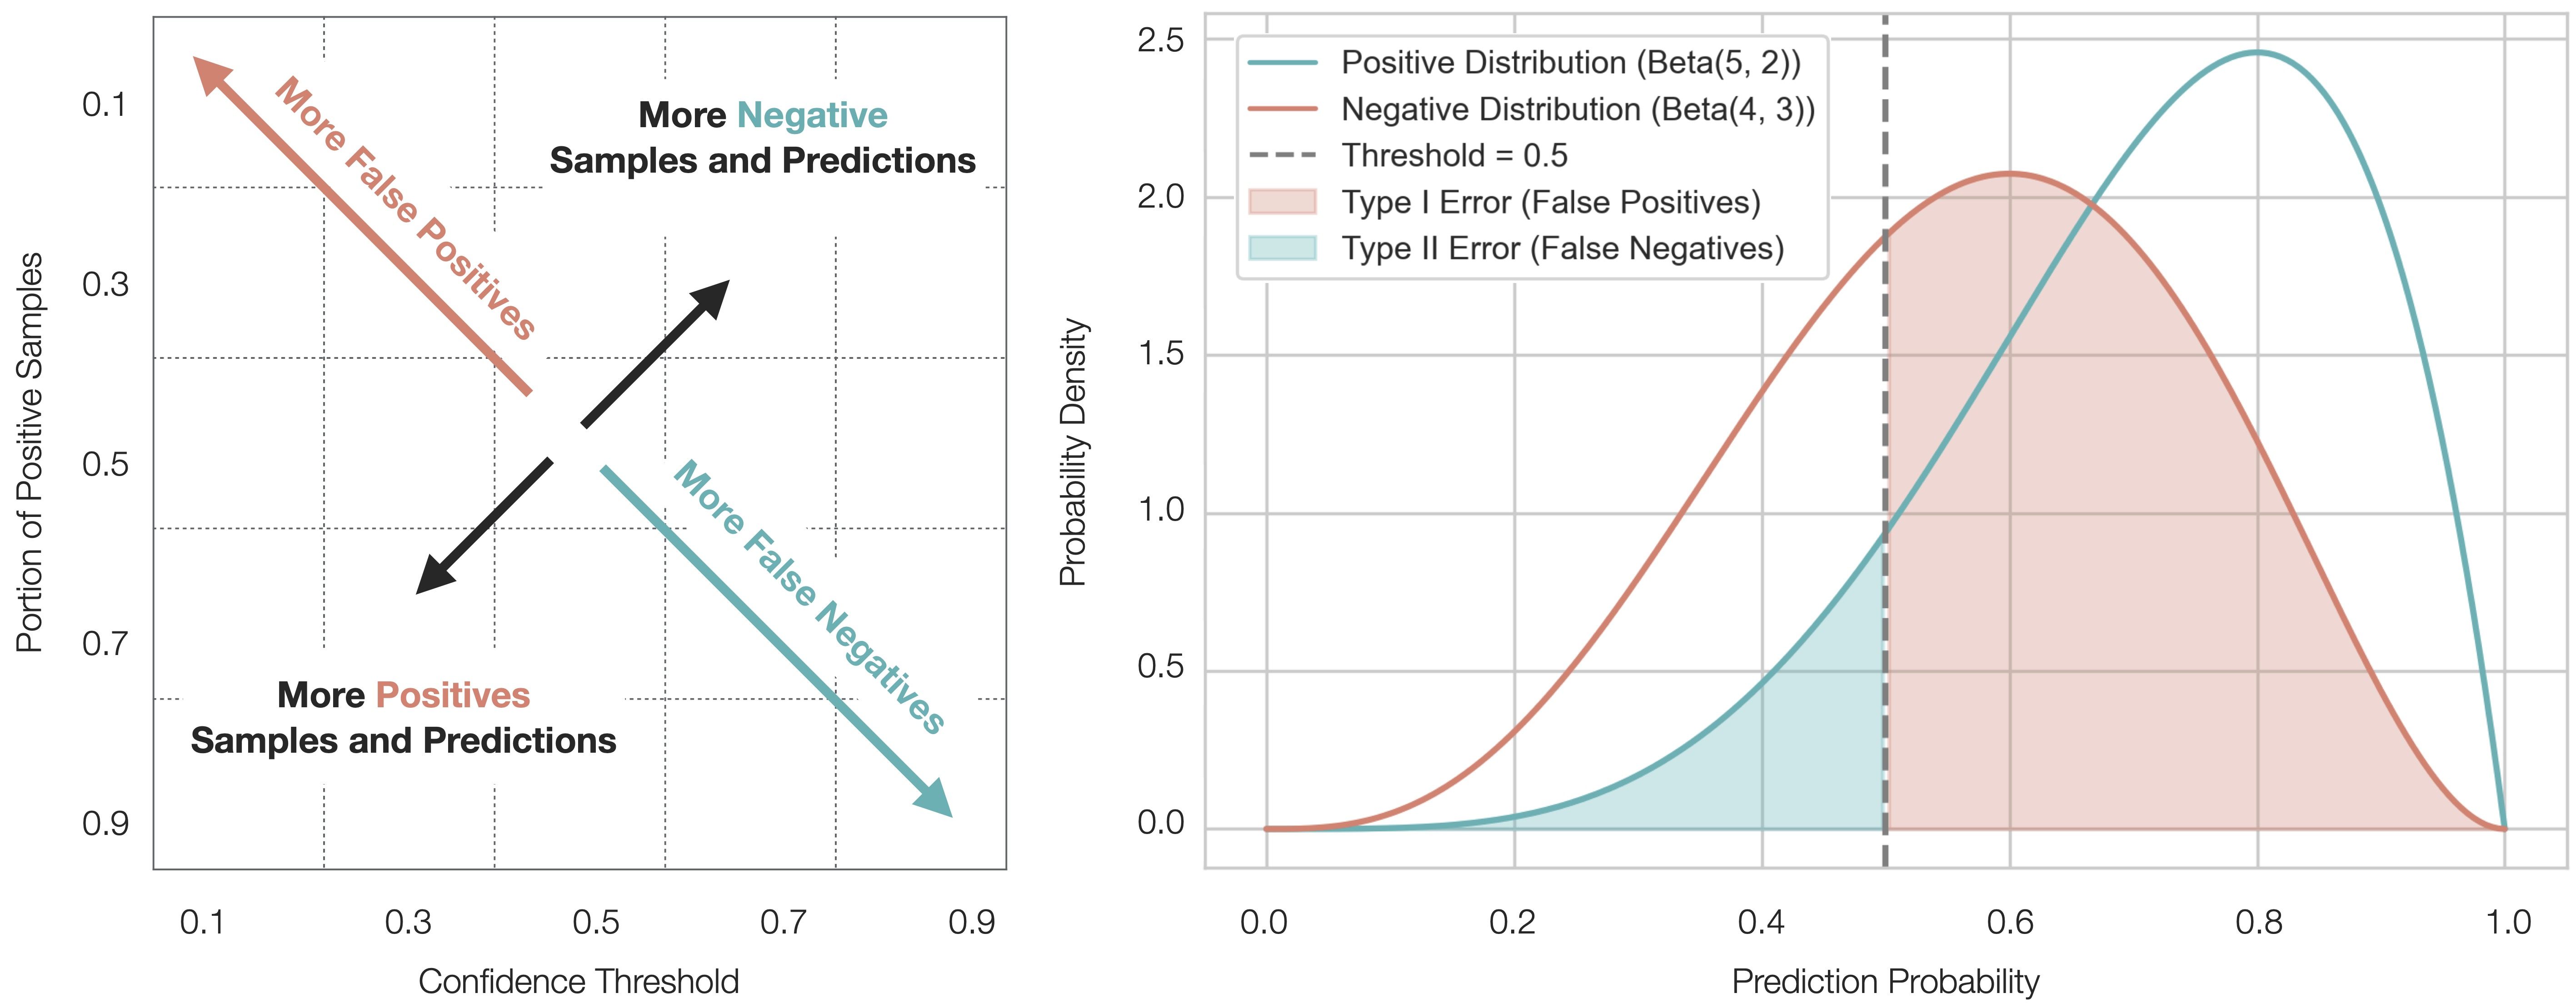
\includegraphics[width=1\textwidth]{fig_5.jpg}
    \caption{Illustration of the simulation design for evaluating classification metrics under varying balance and confidence thresholds. (Left) A 5 × 5 grid of performance metrics, with each cell representing a unique combination of balance level and confidence threshold. (Right) The prediction probability distribution for positive and negative samples.}
    \label{fig:s5_classification}
\end{figure}

The objective of this experiment is to investigate two critical aspects of evaluating binary classification models: the balance between positive and negative samples and the choice of confidence threshold. The experiment aims to explore how these factors influence the performance metrics used to evaluate classification models and to provide insights into the necessity of reporting specific metrics together.



To achieve this, five levels of balance and five levels of confidence thresholds are examined, forming a total of 25 combinations. The inspected levels are $[0.1, 0.3, 0.5, 0.7, 0.9]$ for both balance and confidence thresholds. The balance level is determined by the proportion of positive samples, with a balance level of 0.9 indicating that 90\% of the samples are positive. The confidence threshold is used to dichotomize prediction probabilities, where a higher threshold results in fewer positive predictions by requiring higher certainty for a positive classification. This simulation produces a 5 × 5 grid of performance metrics, where each cell represents a unique combination of balance and confidence threshold (Figure ~\ref{fig:s5_classification}a). The top-left corner of the grid corresponds to a scenario where positive samples are rare, and the model uses a low confidence threshold, resulting in a high false positive rate. In contrast, the bottom-right corner represents a scenario where positive samples are abundant, and the model applies a high confidence threshold, leading to a high false negative rate. This design contrasts these two extreme cases and hence provides a comprehensive evaluation of performance metrics across varying conditions.

The prediction probability, which represents the likelihood of a given sample being classified as positive by the model, is simulated using a beta distribution (Figure ~\ref{fig:s5_classification}b). For positive samples, the prediction probability is drawn from a beta distribution with parameters $\alpha = 5$ and $\beta = 2$, resulting in a peak probability around 0.8. 

For negative samples, the beta distribution has parameters $\alpha = 4$ and $\beta = 3$, with a peak probability around 0.6. This design create a scenario where more false positives are expected than false negatives, as the negative samples have high prediction probabilities that overlap with the positive samples. The shaded area in Figure ~\ref{fig:s5_classification}b represents the overlap between the two distributions, where the confidence threshold is applied. This overlap introduces two types of errors: the region to the right of the threshold intersecting with the negative distribution represents false positives (Type I error), while the region to the left of the threshold intersecting with the positive distribution represents false negatives (Type II error). This setup highlights the trade-off between these error types based on the choice of the confidence threshold.

The metrics evaluated in this experiment include TPR, TNR, FPR, FNR, sensitivity, specificity, precision, recall, accuracy, F1 score, F2 score, and MCC. Although some of these metrics are mathematically equivalent but referred to by different names, this experiment also highlights the reasons why certain metrics are commonly reported together and discusses their complementary roles in evaluating model performance.
